% !TeX spellcheck = en_US

\documentclass[10pt,twocolumn,a4paper]{article}
\usepackage{styles/usenix-style}

\author{Fabian Nguyen}


\usepackage{cite,xspace,ifthen,graphicx,listings}
\usepackage[font=small,labelfont=bf]{caption}
\usepackage[
   pdfauthor={Fabian Nguyen},
   pdftitle={Advanced Exploit Mitigation},
   pdfsubject={Windows Internals},
   pdfkeywords={Security,Stack Buffer Overflow,Return Oriented Programming, Control Flow Guard, Shadow Stack}
]{hyperref}
\usepackage[nonumberlist, section]{glossaries}
\usepackage{xurl}
\usepackage{hyperref}

\begin{document}

\title{Windows Internals: Advanced Exploit Mitigation}

\maketitle


\begin{abstract}
We take a look at general techniques used by attackers to compromise Windows systems and some fundamental defense mechanisms against them.
This paper will provide an overview of Microsoft's latest additions to the security concept of the Windows operating system (OS), analyze inherent flaws in their design and take a brief look at already existing attacks. 
\end{abstract}

\section{Introduction}\label{sec:introduction}
In an increasingly digitized world an overwhelming amount of private and/or safety-critical information and data is stored on computers.
Windows is by far the most used operating system on desktop PCs \cite{OSshare} and therefore a main target of attackers to compromise data or computer systems.
A common intent of attackers is to steal an individual's private/confidential data or to install ransomware to extort money.
Naturally, as the amount and complexity of attacks rise, OS vendors are forced to put an increasingly high amount of effort into mitigating existing weaknesses and deny attackers  further possibilities to compromise the OS.
Even though this is the case, the amount of potentially abusable vulnerabilities in Windows has been increasing, instead of decreasing.

\begin{figure}[h]
\centering
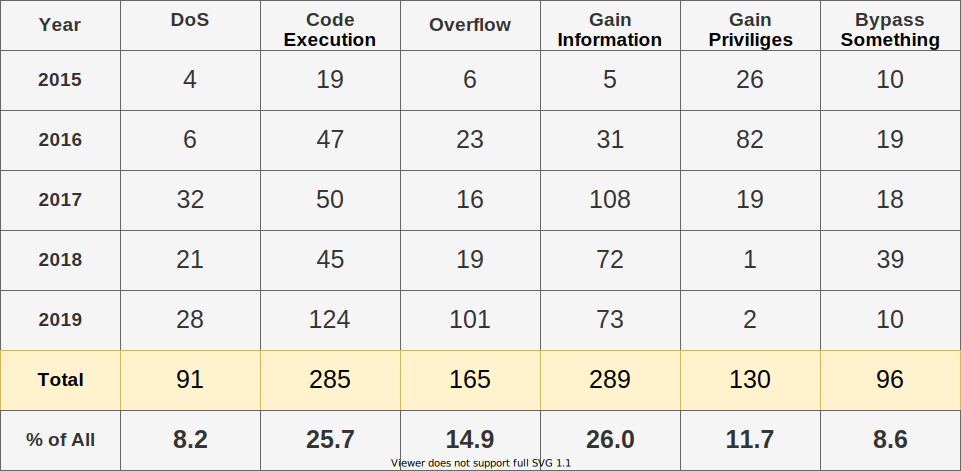
\includegraphics[keepaspectratio,width=\linewidth]{fig/cve}
\caption{Amount of documented vulnerabilities in the Windows operating system (XSS with 0.3\% share omitted for clarity)\textsuperscript{\cite{CVE}}.\newline Note that the spike in \emph{Gain Information} vulnerabilities in 2017 is inflated by a family of attacks widely known as Meltdown/Spectre.}
\end{figure}
\newpage
In figure 1, we can see that the three largest groups of vulnerabilities consist of \emph{Gain Information}, \emph{Code Execution} and \emph{Overflow}.
These three categories are not entirely separated from each other.
An attacker that is able to execute code on a machine often does so in order to gain information and overflows are often the reason why an attacker can execute code in the first place.
We will take a look at how these issues play together and what has been done against them in the past before taking a deeper dive into Microsoft's newest defense additions.

\section{Techniques and Data of Interest}
More specifically, we will analyze Microsoft's two pillars of "Control-flow Enforcement" called control flow guard (CFG), which aims to protect forward jumps (calls), and shadow stacks (SS), which aim to protect backward jumps (returns)\cite{SS}.  Before doing so, we will take a look at why such sophisticated technologies are needed in the first place and what has been done in the interest of security before.
Both of these technologies and relevant underlying concepts, namely overflows, ASLR, DEP, and ROP, will be explained, followed by a further going analysis of  strengths and weaknesses of CFG and SS, i.e. runtime and performance overhead as well as vulnerabilities and evaluation of design choices,  and mentioning of existing attacks where applicable.

\section{Index}
Section 3 will describe overflows, which frequently cause vulnerabilities to exist in the first place, are a building block of further techniques and will therefore be explained first.
We will continue with a quick look at data execution prevention as a countermeasure against some attacks abusing overflows and an advanced form of these attacks in sections 4 and 5, respectively.
Section 6 will deal with address space layout randomization, another attempt to address these attacks.
Our main focus lies on Section 7 which explains the concept of shadow stacks and Section 8 which explains the control flow guard. Both of them will be followed by an evaluation.
Lastly, Section 9 will contain a conclusion of the discussed topics.

\section{Overflows}\label{sec:Overflows}
An overflow happens when a program writes data to memory beyond the limits of the underlying data structure.
One common example of this is a stack buffer overflow caused by an incorrect use of the function \texttt{strcpy()}\footnote{\texttt{char * strcpy ( char * destination, const char * source )} is a C function that copies a string into the specified destination buffer}.\newline
More precisely, an overflow can occur when the given input is longer than the buffer one writes to, as seen in figure 2.
\begin{figure}[h]
\centering
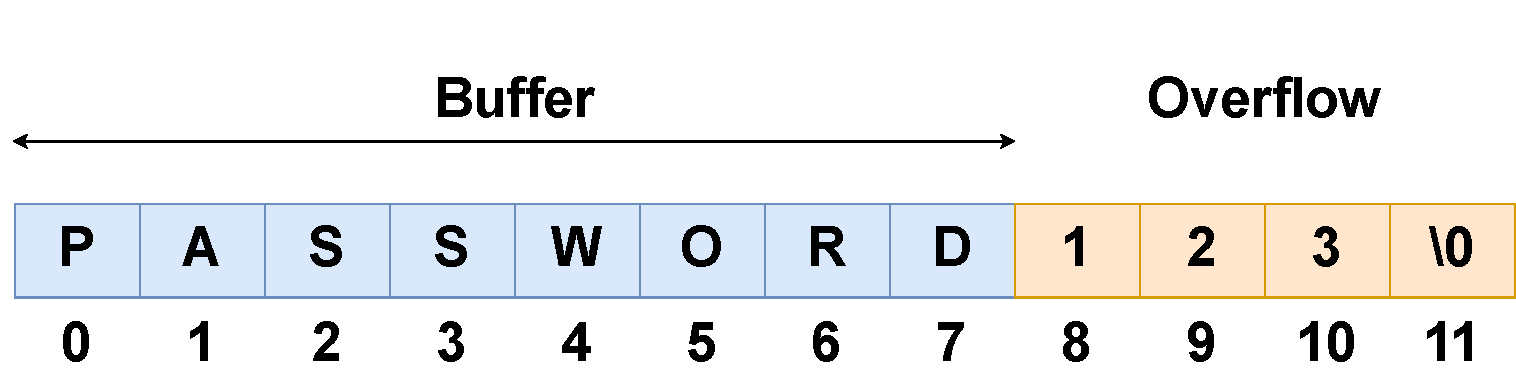
\includegraphics[keepaspectratio,width=\linewidth,trim={0 0 0 1.5cm}]{fig/simpleoverflow}
\caption{The password's length is too large to fit into the designated buffer. However, \texttt{strcpy()} will not check for valid sizes so it will continuously write beyond the buffer}
\end{figure}\newline
Relatively small-in-size overflows are not always easy to spot and often remain unidentified if they do not cause immediate errors.
In addition to causing faulty program behavior, this also provides a critical attack surface.
To see why this is the case let us take a look at a typical stack layout with only one buffer present right at the beginning.
\begin{figure}[h]
	\begin{center}
		\centering
		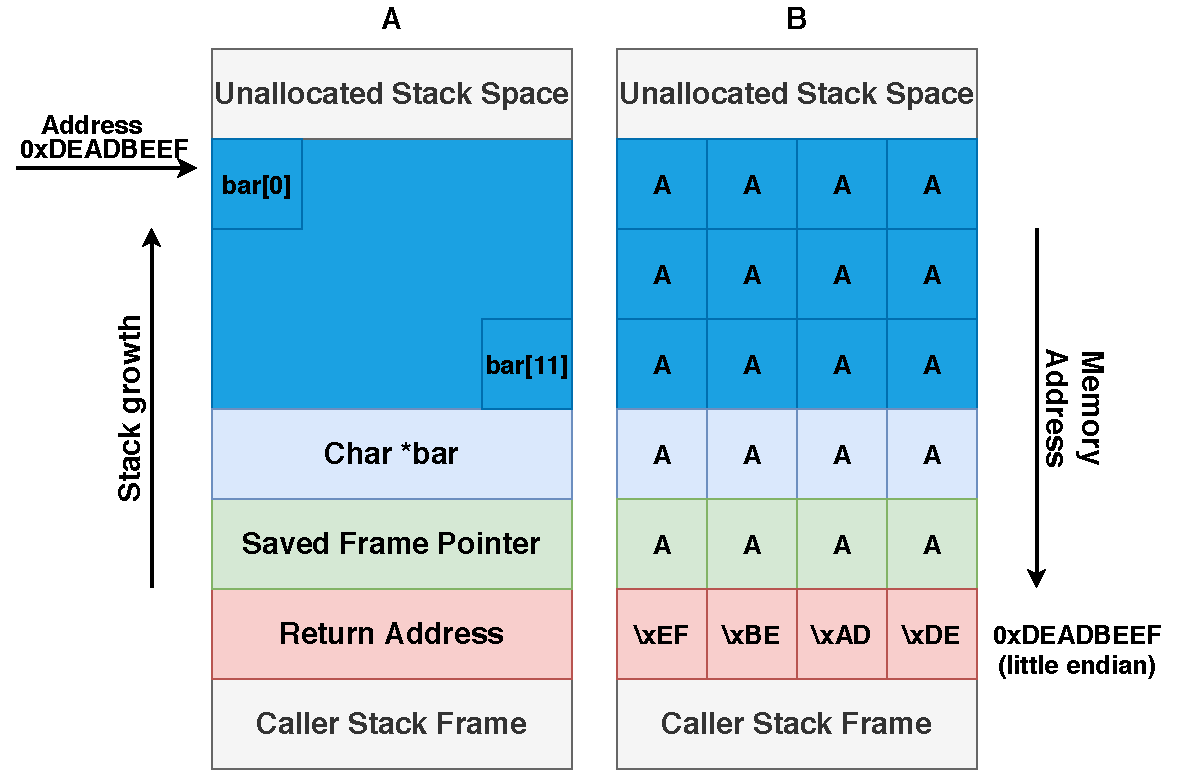
\includegraphics[keepaspectratio,width=\linewidth,trim={1cm 0 1cm 0}]{fig/Stacks}
		\caption{ A: Typical Stack Layout after allocating a local buffer within a function with no arguments. \newline B: The same stack after a misuse of \texttt{strcpy()}\textsuperscript{\cite{wiki}}}
	\end{center}
\end{figure} 
\newline
As we can see in Figure 3 (A) the stack will usually contain a return address right at the bottom, a frame pointer on top of it, and then local data that is used by the current function.
One will also need to keep the parent function's data saved below (stack grows upwards in this example).
There is only one character buffer of size 12 and a pointer to it.
Suppose one wants to copy a user-input string into this buffer e.g., by using \texttt{strcpy()}.
The user may now unknowingly or perhaps purposely overflow this buffer by entering a string that is longer than 12 characters.
As we observed earlier this will result in a memory write beyond the buffer's bounds. 
Figure 3 (B) shows how the same stack might look after an overflow occurred. We can see that our pointer to the buffer is overwritten, as well as the frame pointer we had saved on the stack earlier.
Most importantly though, the return address is also corrupted.
In the given figure, the input is constructed so that the part that is written over the return address resembles an address itself.
In this case, it is just the address of the buffer again.
At some point, our given function will attempt to return to this address.
However, once it does so, all it will be able to read from this address is a string of 'A's which certainly does not resemble a valid sequence of code.
The program will fault and terminate.
This problem has existed for as long as the concept of the stack itself, so naturally techniques to (try) prevent this from happening were implemented long ago.

\section{Data Execution Prevention}\label{sec:DEP}
One intuitive way to address the unintended execution of (possibly injected) code on the stack is the use of Data Execution Prevention (DEP).
DEP follows a very simple approach to prevent the execution of code from malicious addresses.
Note that an attacker that uses (stack-/heap) overflows can only manipulate memory which is typically used for non-executable data.
Based on this assumption, we could mark the entire stack/heap memory(with an additional attribute for memory pages) as \emph{non-executable} or "NX" in short\footnote{Sometimes a program, e.g. a Just-in-Time compiler, needs to generate code directly into memory, so this is a very simplified approach.}.
Whenever an attempt to run code is made a check will ensure that the "NX"-Bit for the according page is not set. If it is, the program will terminate\cite{DEP}.
This approach offers an easy solution to prevent the \emph{execution} of code on the stack.
However, it does \emph{not} prevent an attacker from redirecting control flow to already existing code. Attacks that abuse this flaw could therefore still compromise or even take over a program.\footnote{A well-known way to do this is a \hyperref{https://en.wikipedia.org/wiki/Return-to-libc_attack}{Return-to-Libc Exploits}{name}{return-to-libc attack}.}

\section{Return-Oriented Programming}\label{ROP}
Return-oriented programming describes one of the most popular approaches to manipulating programs by hijacking control flow through the manipulation of return addresses.
In essence, there are three steps to do:
\begin{enumerate}
	\item Finding a security vulnerability that allows one to manipulate memory
		\item Writing code (also called payload or shellcode)\footnote{The name shellcode comes from the fact that such attacks often inject code to open a shell on the target system} on the stack 
	\item Manipulating the return address to point to the injected code
\end{enumerate}
Windows did not offer any kind of protection against ROP attacks until 2004 when DEP was introduced.
However, as already mentioned, attackers quickly overcame this barrier by using already existent code which would not be marked non-executable\cite{solar}.
A change to the calling convention that should have theoretically stopped this from happening was to require function arguments to be passed in registers instead\cite{calling}. Registers are not as easy to manipulate due to not being as easily writable per overflows, though attackers easily overcame this restriction as well.
Instead of using complete functions they would now use only small portions of a function\cite{krahmer}. Naturally, instruction sequences that allowed to manipulate registers were especially useful, in order to invoke complete functions again.
However, this is not needed as the usage of such so called "gadgets" is already turing-complete\footnote{A system is called turing-complete if it is able to simulate any Turing machine. In essence, this means that it is "fully functional" in a computational sense, as most programming languages and systems are\cite{Turing}.} given a \emph{big enough}\cite{gadgets} program.
This is made even easier by the fact that one can use instruction sequences that were not supposed to be in the program to begin with.
To see how this is possible, recall how machine code is written and read by the CPU.
Note that in contrast to natural language, machine code does not include any white space (e.g., spaces or slashes) so one may start reading wherever they want\cite{gadgets}.
Figure 4 shows an example where two instructions are split into four just by removing one byte at the start.
\begin{figure}[h]
  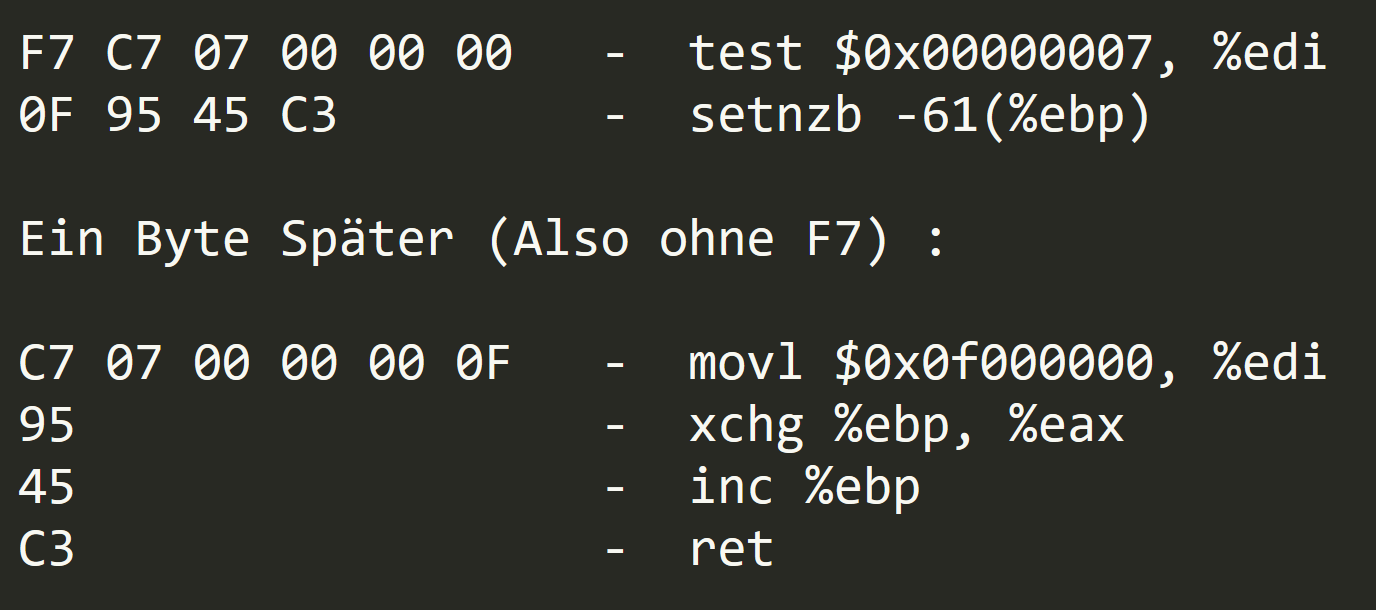
\includegraphics[keepaspectratio,width=8cm]{fig/ByteCode}
  \caption{An example of an unintended use of machine code\textsuperscript{\cite{geometry}}. Ignoring the first byte results in a sequence of four instructions instead of two}
\end{figure}\newline
Note that the resulting instruction sequence ends with a \texttt{ret}, which allows us to continuously chain such gadgets.
We can easily find such sequences by searching for \texttt{ret} instructions (in this example, the byte C3) and then going as far back as useful instructions follow\cite{gadgets}.

\section{Address Space Layout Randomization}\label{sec:ASLR}
Address Space Layout Randomization (ASLR) was implemented to address this issue.
Since an attacker that uses preexisting code needs to be able to tell where the code they want to use is, an easy solution is to prevent them from addressing said code.
ASLR does this by randomizing the arrangement of segments like the stack, heap, and DLLs in memory\cite{ASLR}. This means that using a fixed address to reference memory will most likely result in a segmentation error or the wrong code being targeted at best.
In theory, ASLR should prevent ROP attacks completely since no attacker should be able to locate any specific code to begin with.
However, a single pointer leak may compromise the location of any of the segments and thus break ASLR completely\cite{bypass}. Note that 64-bit compiled programs have an advantage over 32-bit ones here as Windows can randomize 8 of the address' bits for 32-bit programs and a total of 17/19 bits (.exe/.dll) for 64-bit ones.\cite{ASLRBits2}
Furthermore, ASLR on its own is not particularly good at preventing attacks as brute-forcing is still a viable attack. In a 64-bit DLL there are 524288 (2\textsuperscript{19}) possible base addresses for ASLR to choose from\cite{ASLRBits}. Assuming that the attacker is able to make 10 guesses per second (which isn't a high requirement with modern CPUs), this gives us a time span of a about 15 hours at best.
Hence, developers should try to detect brute-force attacks and avoid practices that make them feasible. An example of this is to not automatically (and/or instantly) restart a crashing process\cite{ASLRBits}.
Consequently, vulnerabilities in both DEP and ASLR (even combined) have been found and successfully exploited\cite{bypass}\cite{ASLRBits2}.
How this was done will not be covered in this report, but it is important to see that these techniques were not sufficient protection after all.

\section{Shadow Stack}\label{shadowstack}
The idea of a shadow stack follows a different approach to the issue.
Instead of trying to prevent the manipulation of the return address, an additional check is built-in to make sure it was not altered.
In order to do this, the shadow stack saves a copy of all return addresses in a separate memory location\cite{shan}.
Every \texttt{call} instruction in a program pushes the return address of the parent routine on the normal stack \emph{and} on the shadow stack.
Every return instruction pops one address off the shadow stack and compares it to the address on the normal stack\cite{shan}.
\begin{figure}[h]
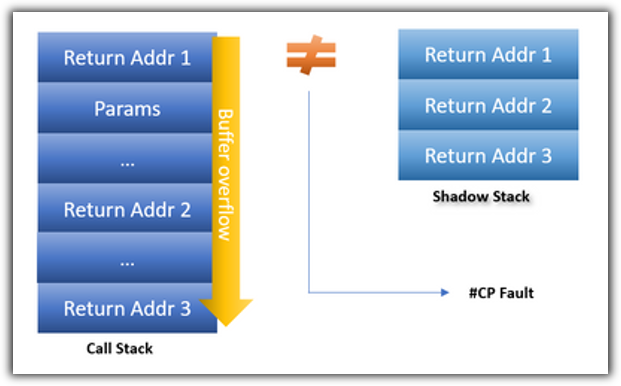
\includegraphics[keepaspectratio,width=8cm]{fig/ShadowStack}
\caption{Shadow Stack Overview. Every return address on the stack is matched by a copy of that return address on the shadow stack.}
\end{figure}

In order to implement this check, a new register called shadow stack pointer(SSP) and an additional memory page attribute are used.
Writes to the shadow stack are restricted to control transfer instructions (\texttt{call/ret)} and shadow stack management instructions\footnote{There is no point in having a separate stack to save data when its explicitly writable.}\cite{CFE}.
Note that calls to exception handlers and \emph{longjmp}s may cause issues as calls and returns are not necessarily perfectly matched if they occur\cite{light}.
One solution to this is to continuously pop addresses off the shadow stack until a matching address is found. In this case, a program would be terminated if the shadow stack runs empty without match\cite{performance}.
Implementing special treatment for these troublesome calls instead could increase runtime performance but include a higher memory overhead and increase complexity.
Using a parallel shadow stack removes the necessity of considering mismatches between \texttt{call/ret} instructions as unexpected changes to the stack pointer (i.e \% esp) are implicitly matched\cite{performance}.
Parallel shadow stacks are placed at a fixed offset relative to the main stack and all return addresses are placed parallel to the return addresses on the main stack (hence the name parallel shadow stack). 
As a consequence of this, parallel shadow stacks have drastically reduced performance overhead (generally less than half), as it is no longer necessary to maintain the SSP (i.e copying it to/from memory), but sacrifice some security to achieve this result\cite{performance}.
Note that shadow stacks only provide integrity of "backward jumps" (also called backward edges)."Forward jumps" may still be manipulated while a shadow stack is being used.
\subsection{Shadow Stack Revisited}
One main problem with the shadow stack is that no one (except for researchers and employees that have early access to hardware that is still in development) is able to make use of it as of now. Since Microsoft's implementation of the shadow stack requires an additional register, it is only usable with certain CPUs (more specifically those using a chipset that supports Intel Control-Flow-Enforcement technology)\cite{CFE}.
Intel's first generation of CPUs that use this chipset are yet to be released\footnote{Intel Tiger Lake CPUs are announced for late 2020} and so are AMD's.
\newline ARM will not be releasing any compatible CPUs\cite{techrepublic}.
Additionally, once compatible CPUs are released it will still take a couple of years for them to be used widely.
Considering that a software version of the shadow stack dubbed Return Flow Guard (RFG)\cite{RFG} was already in development, it is not quite apparent why this approach was not further pursued to bridge the time needed for hardware shadow stacks to spread.
According to unofficial sources, development of the RFG was discontinued because a vulnerability (more specifically, a race condition) in the implementation was found\cite{techrepublic}.
Performance overhead can range from as low as 3.5 (parallel) to roughly 10\% (traditional shadow stacks)\cite{performance}. As Microsoft's implementation of the shadow stack will be neither parallel (since a SSP is used) nor a basic traditional shadow stack we can expect the overhead to be anywhere in between these bounds.
Note that the shadow stack only validates return addresses. Function parameters are (intentionally) not protected\cite{SS}.
Considering that it is unlikely for an attacker to be able to manipulate a function's parameters in between the call and the function running, this makes sense. Even if one were to try protecting them, it is unclear in which order the parameters should be saved to the shadow stack as the order of their use may be undetermined. It would also require doing this check for their first use only as they may be legitimately altered within the function.
Lastly, according to Microsoft, the use of shadow stacks will be opt-in "at first" per linker-flag for apps and DLLs for compatibility reasons\cite{SS}. This will further increase the time needed for the shadow stack to spread.

\section{Control Flow Guard}\label{CFG}
To take care of the forward edges Control Flow Guard was shipped with Windows 8.1 Update 3\cite{cfgexplore}.
More specifically, CFG aims to prevent the misuse of indirect jumps.
To do this, developers can compile their programs with the CFG flag and ensure that their program will only run on memory areas that have been marked "safe" earlier\cite{CFG2}.
Here, "safe" means that the address of every indirect jump refers to a valid function in the program.
In order to check this efficiently at run time, a bitmap of the starting addresses of every function is created at compile time where every bit in the bitmap corresponds to 8/16 \footnote{1 bit per 8bytes at first, changed to 2 Bit-Tuple per 16 bytes later} bytes in the address space\cite{cfgexplore}.
If a function starts within the block of addresses that correspond to a given bit it is set to '1', otherwise it is '0'.
A guard instruction is then inserted before every indirect jump which validates that the matching bit for the target address in the bitmap is set to 1 (see figures 6 and 7)\cite{cfgexplore}. If it is not, a Control-Protection Exception is thrown and the program is terminated immediately\cite{SS}.
\begin{figure}[htbp]
	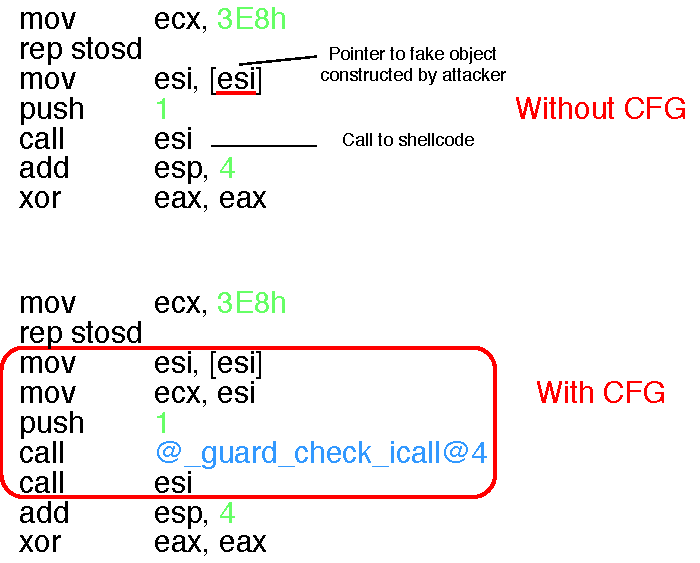
\includegraphics[keepaspectratio,width=8cm]{fig/cfg}
	\caption{Example code with/without CFG enabled\textsuperscript{\cite{cfgexplore}}}
\end{figure}
If a CFG compatible program is run on a Windows version that does not support CFG the call \texttt{\textunderscore guard\textunderscore check\textunderscore icall} (as seen in figure 7) will run a function that does nothing, otherwise it will point to \texttt{ntdll!LdrpValidateUserCallTarget} which takes the target address as argument and performs the bitmap validation\cite{cfgexplore}.
To increase performance, system processes which are run as "protected" processes use shared bitmaps for DLLs.
This means that per DLL only one bitmap is needed for all protected processes unless a process tries to alter the bitmap. In this case, the bitmap is mapped into the process' private memory\cite{cfginternals}.
Note that dynamically generated functions cannot be protected this way as explicitly allocated and \emph{executable} marked memory has its corresponding bits in the bitmap implicitly set to 1\cite{cfgexplore}.
This is because dynamically allocated memory cannot be considered at compile time.
\subsection{Control Flow Guard Revisited}
One major flaw in the initial design of CFG lies in one of its main assumptions: That the addresses of functions are aligned to eight bytes.
While this assumption holds true for the compiled program itself (since the compiler can enforce the alignment) it certainly does not for DLLs.
To make up for this issue, CFG uses a mapping of two bits (a tuple) for every 16 bytes since Windows 10 instead, where (0,0) means no function starts in the corresponding address block, (1,0) means a function starts at the start of the block, and (1,1) means a function starts anywhere in the block\cite{tuple}.
\begin{figure}[h]
	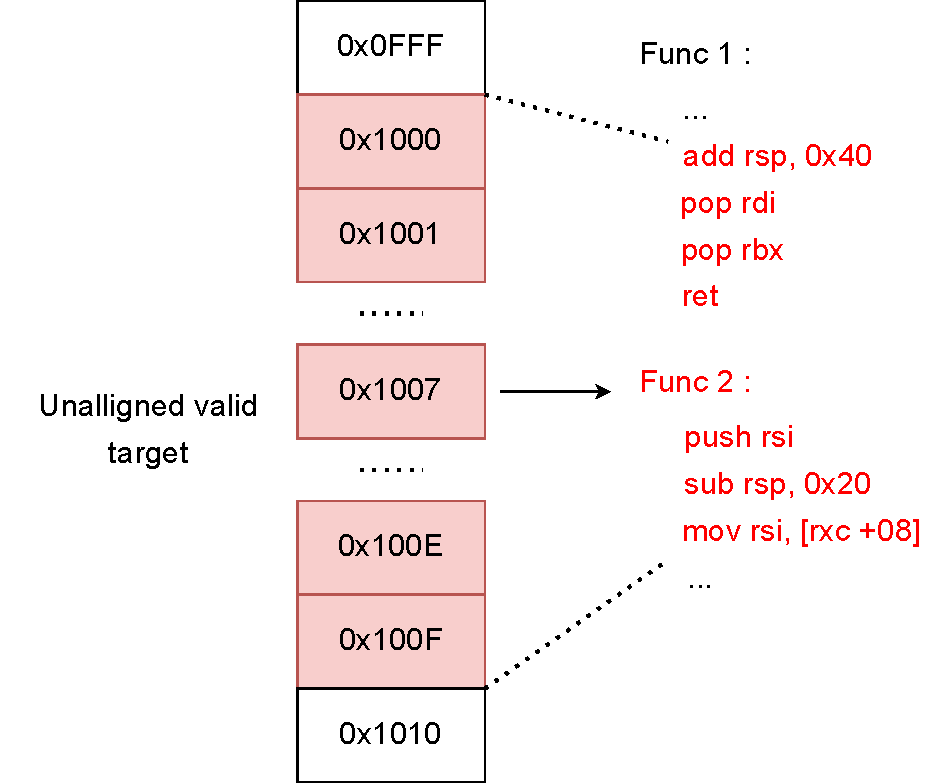
\includegraphics[keepaspectratio,width=\linewidth]{fig/unallignedcode}
	\caption{An example of why unaligned addresses can be a major vulnerability. Func2 makes the whole 16 byte range from 0x1000 to 0x100F valid, which contains instructions of func1's epilogue\textsuperscript{\cite{cfgexplore}}}
\end{figure}\newline
Note that this still provides a sort of margin for attacks when alignment is not enforced as an attacker can still manipulate a jump to point to anywhere within a (1,1) block (15 bytes of unintended viable targets in the worst case!).
This is demonstrated in figure 8.
This has detrimental consequences, as lots of even Windows' own system DLLs are not compiled to use CFG and therefore not (necessarily) aligned properly (145 in Windows 10 1511 / still 50+ in build 18362\cite{cfgbypass2}).
Note that any module, even if it is compiled to use CFG, is vulnerable when it is used by a program that is not, since CFG will be disabled in the entire process\cite{cfgexplore}.
Similarly, any process that uses a DLL without CFG is vulnerable as all addresses within said DLL will be allowed\cite{cfgbypass2}.
Another oversight that was found rather quickly: The guard function was not properly protected in early CFG versions.
In 2015 Zhang Yunhai showed that by using a (custom-) heap-allocation and freeing it afterwards,  it was possible to make its memory area writable again under certain circumstances\cite{cfgbypass}.
Attackers were therefore able to edit its contents and consequently allow all calls.


\section{Conclusion}\label{sec:conclusion}

While both control flow guard and shadow stacks are valuable additions to the Windows security concept, Microsoft's war on hackers is far from over. As we have seen, CFG offers significant protection for forward edges only in optimal circumstances, is therefore vulnerable by design and has already been bypassed multiple times. The shadow stack has not been enabled for widespread use in Windows yet, so its impact remains to be seen. Even if significant vulnerabilities exist (which is likely) it will still place a burden on attackers to find and exploit them successfully.
Nonetheless, performance (and possibly memory-) overhead may greatly impact the time needed for the shadow stack to be used widely and may well be a hindering factor for its spread.
Microsoft will have to continuously monitor and refine their implementations (and in case of CFG their \emph{application}) of these techniques to fix vulnerabilities, reduce attack surface and encourage widespread use of them.


\bibliographystyle{ieeetr}
\bibliography{AdvancedExploitMitigation}


\end{document}